\documentclass[11pt]{report}
\usepackage[margin=2cm]{geometry}
\usepackage{graphicx}
\usepackage{hyperref}
\usepackage{amsmath}
\usepackage{amssymb}
\usepackage{upgreek}
\usepackage{amsmath,amssymb,amsthm,textcomp, stmaryrd}
\usepackage[english]{babel}
\usepackage[autostyle]{csquotes}
\usepackage[document]{ragged2e}
\usepackage{hhline}
\newcommand{\uline}[1]{\rule[0pt]{#1}{0.4pt}}
\newcommand{\sqheader}[2]{
    \normalsize {San Quentin Math Circle // #1}
    \begin{center}
        %% Assignment title
        \textbf{#2}
    \end{center}
}

\begin{document}
   \sqheader{Spring 2019}{Logic Gates 2 - Electric Boogaloo}
 
\begin{center}
	Before we get started on the new logic gates, let's have a quick refresher on what we covered last week: \text{\emph{AND}}, \text{\emph{OR}}, and  \text{\emph{NOT}}. \\Below is a visual representation and truth table of each operator
\end{center}

\vspace{20mm}
\hspace{1in}
\begin{minipage}{.5\linewidth}
    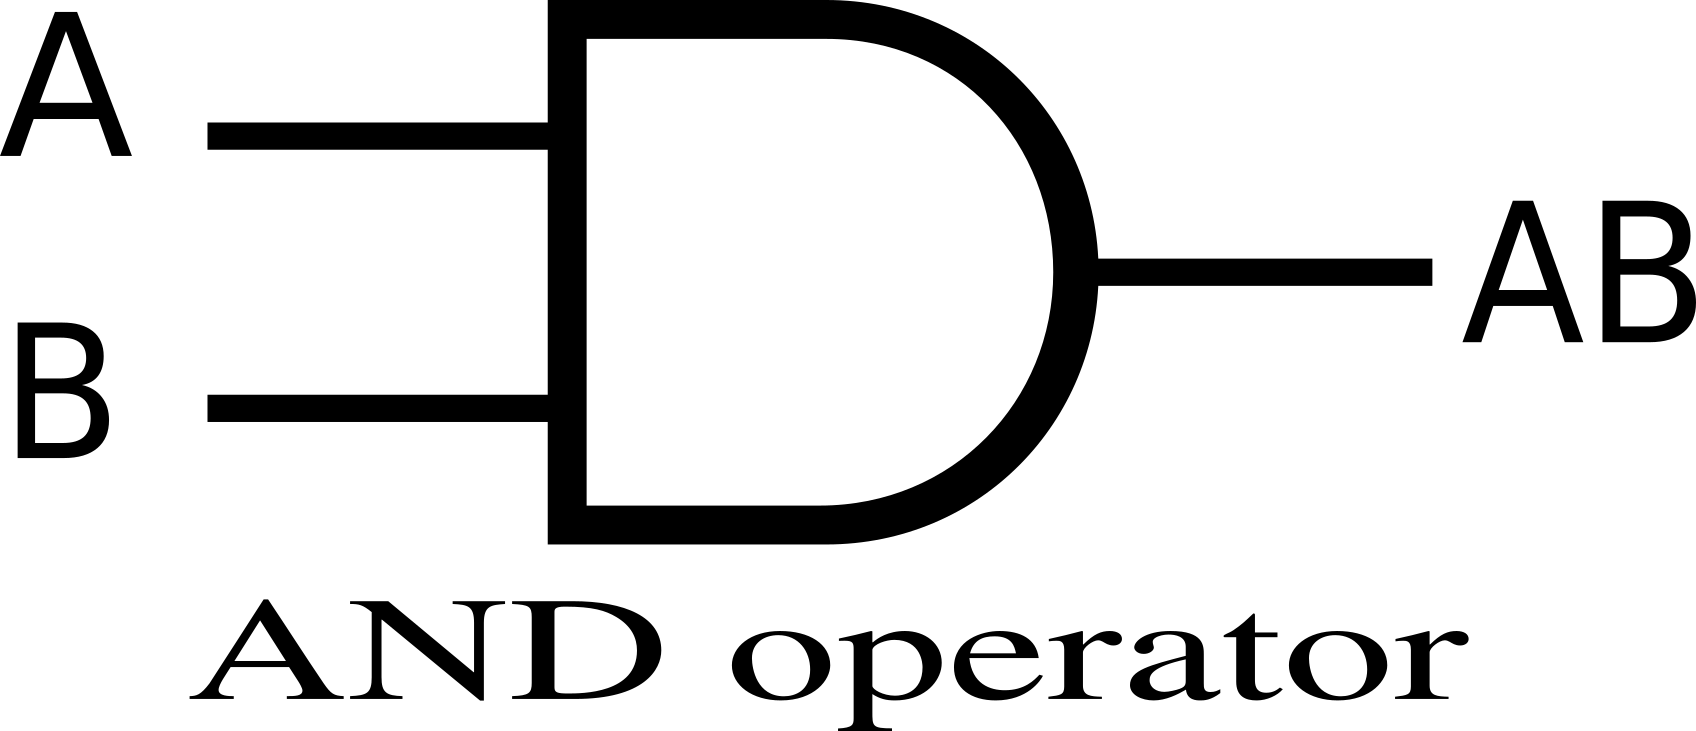
\includegraphics[width=3 in]{images/and.png}
	\label{img2}
\end{minipage}
\begin{minipage}{\linewidth}
\begin{tabular}{|ll|l|}
	\hline
	Input                   &   & Output  \\ \hline
	\multicolumn{1}{|l|}{A} & B & A and B \\ \hline
	\multicolumn{1}{|l|}{0} & 0 & 0       \\ \hline
	\multicolumn{1}{|l|}{1} & 0 & 0       \\ \hline
	\multicolumn{1}{|l|}{0} & 1 & 0       \\ \hline
	\multicolumn{1}{|l|}{1} & 1 & 1       \\ \hline
\end{tabular}
\end{minipage}


\vspace{20mm}
\hspace{1in}
\begin{minipage}{.5\linewidth}
    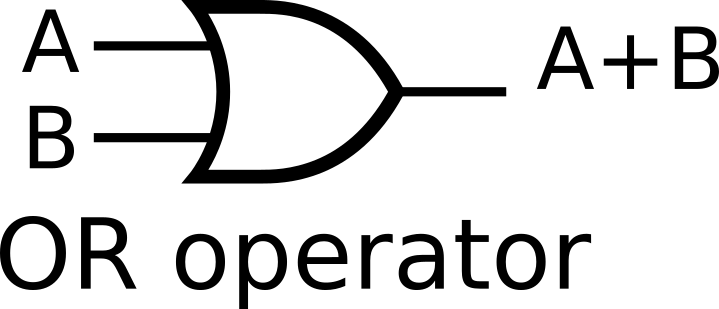
\includegraphics[width=3 in]{images/or1.png}
	\label{img2}
\end{minipage}
\begin{minipage}{\linewidth}
\begin{tabular}{|ll|l|}
	\hline
	Input                   &   & Output  \\ \hline
    \multicolumn{1}{|l|}{A} & B & A or B \\ \hline
	\multicolumn{1}{|l|}{0} & 0 & 0       \\ \hline
	\multicolumn{1}{|l|}{1} & 0 & 1       \\ \hline
	\multicolumn{1}{|l|}{0} & 1 & 1       \\ \hline
	\multicolumn{1}{|l|}{1} & 1 & 1       \\ \hline
\end{tabular}
\end{minipage}


\vspace{20mm}
\hspace{1in}
\begin{minipage}{.5\linewidth}
    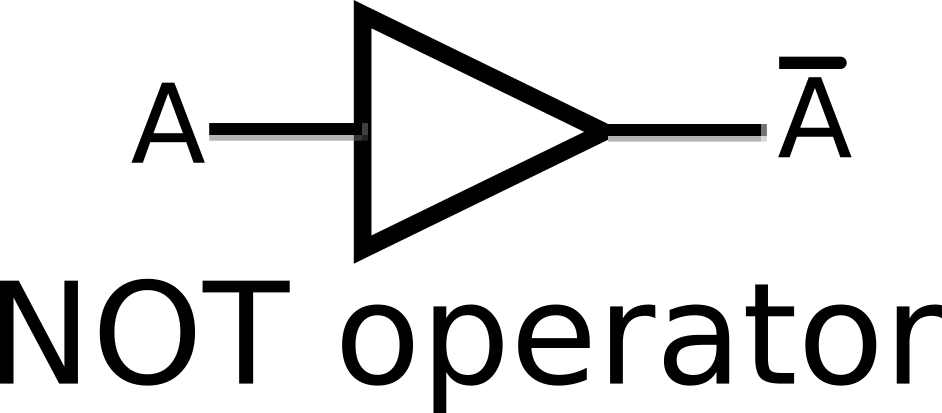
\includegraphics[width=3 in]{images/not1.png}
	\label{img2}
\end{minipage}
\begin{minipage}{\linewidth}
	\begin{tabular}{|l|l|}
		\hline
		Input & Output \\ \hline
		A     & NOT A  \\ \hline
		1 & 0     \\ \hline
		0 & 1     \\ \hline
	\end{tabular}
\end{minipage}


\vspace{10mm}
\begin{center}
	\Large
	\textbf{Commonly Used Symbols}
	\normalsize
	
	A and B $\rightarrow$ A $\wedge$ B or A $\cdot$ B\\
	A or B $\rightarrow$ A $\vee $ B or A + B\\
	Not A $\rightarrow$ $\bar{A}$ or $\neg$ A\\
\end{center}

\newpage
Today, we'll introduce some new logic gates, which are actually just combinations of previous logic gates we've seen so far! The first
two of these, are NAND and NOR. These are made simply by tacking on the NOT logic gate after the AND logic gate, or the OR logic gate,
which is where we get the names from, N(ot)AND, and N(ot)OR.\\
\vspace{20mm}
\hspace{1in}
\begin{minipage}{.5\linewidth}
    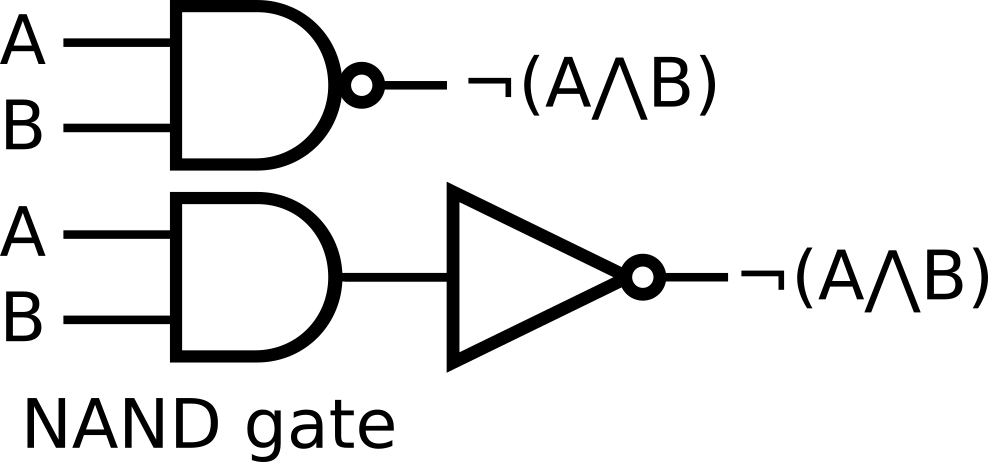
\includegraphics[width=3 in]{images/nand_diagram.png}
	\label{img2}
\end{minipage}
\begin{minipage}{\linewidth}
    \begin{tabular}{|ll|l|}
        \hline
        Input                   &   & Output  \\ \hline
        \multicolumn{1}{|l|}{A} & B & A nand B \\ \hline
        \multicolumn{1}{|l|}{0} & 0 &        \\ \hline
        \multicolumn{1}{|l|}{1} & 0 &        \\ \hline
        \multicolumn{1}{|l|}{0} & 1 &        \\ \hline
        \multicolumn{1}{|l|}{1} & 1 &        \\ \hline
    \end{tabular}
\end{minipage}\\
\vspace{20mm}
\hspace{1in}
\begin{minipage}{.5\linewidth}
    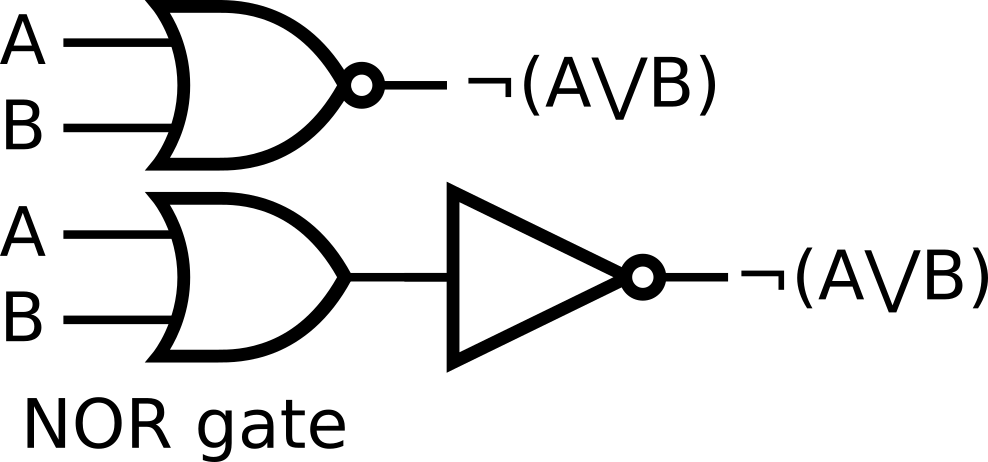
\includegraphics[width=3 in]{images/nor_diagram.png}
	\label{img2}
\end{minipage}
\begin{minipage}{\linewidth}
    \begin{tabular}{|ll|l|}
        \hline
        Input                   &   & Output  \\ \hline
        \multicolumn{1}{|l|}{A} & B & A nor B \\ \hline
        \multicolumn{1}{|l|}{0} & 0 &        \\ \hline
        \multicolumn{1}{|l|}{1} & 0 &        \\ \hline
        \multicolumn{1}{|l|}{0} & 1 &        \\ \hline
        \multicolumn{1}{|l|}{1} & 1 &        \\ \hline
    \end{tabular}
\end{minipage}
\begin{center}
    \textbf{Problems}
\end{center}
    \item Can you think of a real life example of NAND or NOR?
    \vspace{2in}
    \item Can you think of any benefits to making these extra gates?
    \vspace{2in}
\end{enumerate}
\newpage
The next and final gates we'll introduce are XOR and XNOR. XOR is the exclusive or gate, and can be
used to express that two things are mutually exclusive. This is in line with the standard English
usage of or, rather than the math version of or we used last week. Note that we'll introduce
a new symbol for XOR. Following the convention of the previous gates, we'll see that XNOR is the negation
of XOR.\\
\vspace{20mm}
\hspace{1in}
\begin{minipage}{.5\linewidth}
    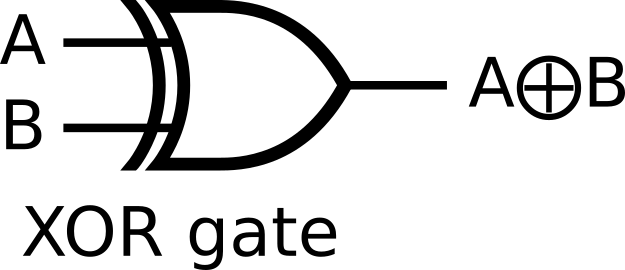
\includegraphics[width=3 in]{images/xor_diagram.png}
	\label{img2}
\end{minipage}
\begin{minipage}{\linewidth}
    \begin{tabular}{|ll|l|}
        \hline
        Input                   &   & Output  \\ \hline
        \multicolumn{1}{|l|}{A} & B & A xor B \\ \hline
        \multicolumn{1}{|l|}{0} & 0 &        \\ \hline
        \multicolumn{1}{|l|}{1} & 0 &       \\ \hline
        \multicolumn{1}{|l|}{0} & 1 &        \\ \hline
        \multicolumn{1}{|l|}{1} & 1 &        \\ \hline
    \end{tabular}
\end{minipage}\\
\vspace{30mm}
\hspace{1in}
\begin{minipage}{.5\linewidth}
    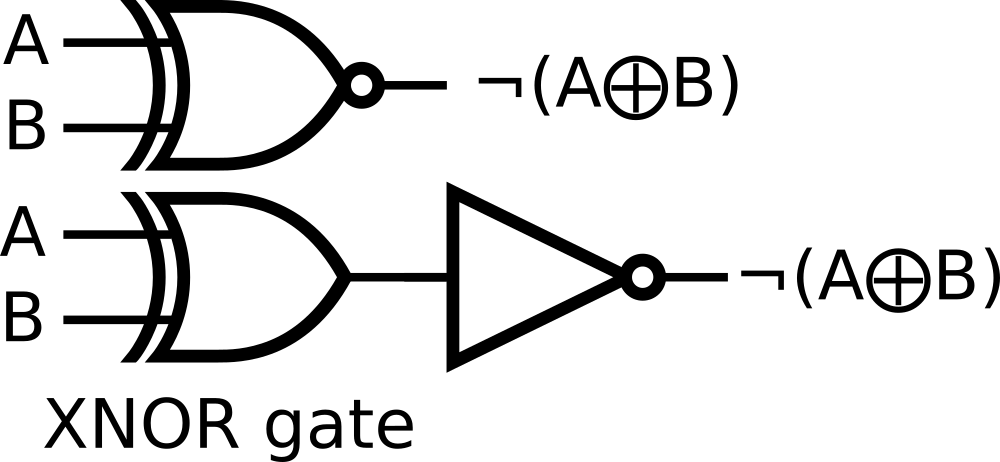
\includegraphics[width=3 in]{images/xnor_diagram.png}
	\label{img2}
\end{minipage}
\begin{minipage}{\linewidth}
    \begin{tabular}{|ll|l|}
        \hline
        Input                   &   & Output  \\ \hline
        \multicolumn{1}{|l|}{A} & B & A xor B \\ \hline
        \multicolumn{1}{|l|}{0} & 0 &        \\ \hline
        \multicolumn{1}{|l|}{1} & 0 &       \\ \hline
        \multicolumn{1}{|l|}{0} & 1 &        \\ \hline
        \multicolumn{1}{|l|}{1} & 1 &        \\ \hline
    \end{tabular}
\end{minipage}
\begin{center}
    \textbf{Problems}
\end{center}
\begin{enumerate}
    \item Can you make a combination of AND and OR gates that replicate the behavior of the XOR gate?
    \item Looking back on all of the new gates, can you see a common reason why there are this many gates?
    \item Can you make a logic diagram with the following truth tables?
    \item Are there any more logic gates that could possibly exist? Explain your reasoning, thoughts or musings on the matter. I encourage
    \item These gates are made to give logic some kind of notation or language which we typically refer to as abstraction. Are there any problems
        with using these to describe any given logical argument or sequence of thoughts? Keep in mind that when we do this kind of thing, our variables
        like A and B from the input columns of each of these diagrams represent a truth, condition or state of existence for some arbitrary thing, like
        last week when we talked about AND in terms of having a cat AND having a dog. Consider the impact of things like varying perspective, and things
        that are not true or not untrue.
        \newpage
    \item All of these questions are optional, but this one is \textit{super optional}. If we consider only the symbols like $\land,\ \lor,\ \neg,\ \oplus$,
        can we give them any of the arithmetic properties we've come to know and love, like commutativity, associativity, and distributivity? Which of
        these properties work with which of these symbols? Recall,
        \begin{align*}
            a+b=b+a&,\ \text{commutativity of addition}\\
            a+(b+c)=(a+b)+c&,\ \text{associativity of addition}\\
            a(b+c)=ab+ac&,\ \text{distributivity of addition}\\
        \end{align*}
        Use the diagrams if they help!
\end{enumerate}
\end{document}

